% 論文誌のルールに従うように注意する。
% * ドキュメントクラスなど: 必ず論文誌が指定しているものを使う。
% * 句読点: 論文誌によって,「,」「。」であったり,「,」「.」あったりする。全角文字と半角文字の使い分けが要求されることもあるので注意。
% * タイトル,著者,日付など: 論文誌によって英文についても記載するようになっていたりと様々。
% * 文献の書き方: 論文誌によっては指定がある。

% \RequirePackage{plautopatch} % エンジンとしてplatex利用時に、パッケージの日本語対応を行う(冒頭に書く)
% (事前に plautopatch をインストールしておくことが必要)

\documentclass[dvipdfmx]{jsarticle}
% \documentclass[dvipdfmx, twocolumn]{jsarticle} % 2段組みにする場合

\usepackage{graphicx} % 画像ファイルの取り込み \includegraphics コマンド

\usepackage{url} % \url コマンド(特殊文字が入ったURLを書きやすくする)

% 上のurlパッケージの代替として、次のhyperrefとpxjahyperを利用すればリンクとして動作するURLを書くことができる。ただし、citesortパッケージと相性問題があり、同時には使えない。
% \usepackage{hyperref} % ハイパーリンク&PDFのブックマーク \href コマンド,\url コマンド
% \usepackage{pxjahyper} % hyperrefを日本語対応させる(文字化けさせない)

\begin{document}

% タイトル,著者,提出日付
\title{象の卵の重さと長径に関する考察}
\author{神谷年洋}
\date{2022年8月1日}
\maketitle

\section{はじめに}

この文書は,レポートや論文の書き方を示すためのサンプルです。
タイトルを「象の卵の重さと長径に関する考察」としてあるのは,あえて荒唐無稽な内容とすることで,
間違えて修正せずに提出されてしまう事故\footnote{参考ツイート \url{https://twitter.com/taku_ymnk/status/392959147974471681}}を防ぐためです。 % footnoteの例
なお,本稿のタイトルを見て``d\'{e}j\`{a}vu''に襲われた方はおそらく研究者だと思われます。 % ダブルクオート、アクセントの利用例

象の卵の存在は現在も未確認であり,その外見については現在も想像するしかない。図\ref{fig:golden_egg}に,想像上の象の卵の外見を示す。 % 図の番号を参照する例

% 図の例
\begin{figure}[htp]
\centering
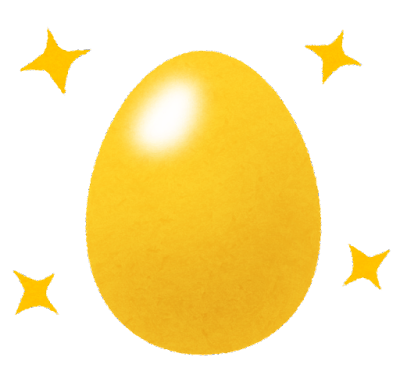
\includegraphics[width=3cm]{golden_egg.png}
\caption{象の卵の想像図}
\label{fig:golden_egg} % 図の相互参照のラベルの例
\end{figure}

\section{関連研究}
\label{sec:related} % 章立ての相互参照のラベルの例。節「関連研究」に「sec:related」というラベルをつけている

象の卵の味覚について,山中\cite{kakenhi_latex}は象の卵が美味しいと言われていることを指摘した。 % 文献の引用の例
象の卵の実在性に関する研究として,寺村ら\cite{teramura2009}は某国の王が実地に象の卵を捜索した事例を報告している。
過去日本にも大陸から象が渡ってきていることが指摘\cite{kamei1990}されており,象の卵が国内で発見される可能性も期待される。

\section{アプローチ}

象の卵を発見するためには,卵の重さやサイズが判明していることが望ましい。
\ref{sec:related}節の関連研究\cite{teramura2009}において象の卵が発見できていないのは,外見上の特徴がわからないために見逃している可能性がある。 % 節の番号を参照する例
本稿では,他の動物との比較により,象の卵の重さやサイズが推定できるのではないかとのアイデアに基づく考察を行う。

\subsection{他の動物のデータを用いた推定}

提案手法は,成体の体重と卵の重さが比例すると仮定し,さらに,卵の重さの$\frac{1}{3}$乗が卵の長径(長軸の長さ)に比例すると仮定することにより,他の動物のデータから象(以下「ゾウ」)の卵の重さとサイズを推定するものである。
表\ref{tab:egg_sizes}に,他の動物とゾウの比較を示す。ゾウの卵の欄については,確認事例がないため空欄としている。 % 表の番号を参照する例

% 表の例
\begin{table}[htbp]
  \centering
  \caption{動物の種類毎の個体や卵のデータ}
  \label{tab:egg_sizes} % 表の相互参照のラベルの例
  \begin{tabular}{|c|r|r|r|}
    \hline
    動物 & 個体の重さ & 卵の重さ & 卵の長軸の長さ \\ \hline \hline
    ニワトリ & 4kg & 60g & 5.5cm \\ \hline
    ガチョウ & 9kg & 150g & 10cm \\ \hline
    ゾウ & 3t & ? & ? \\ \hline
  \end{tabular}
\end{table}

% 表の記述は長く面倒になりがちなので、表の生成をサポートするツールを利用することを推奨します。
% 上の表も VSCode拡張である LaTeX Table Helperhttps://marketplace.visualstudio.com/items?itemName=Lw-lonely.latex-table-helper により作成したものです。

% 文献リストの例
\begin{thebibliography}{99} % 「99」はPDFに表示するときの数字の幅を2桁にするための記述。文献が100個以上あるときは「999」とする。
\bibitem{kakenhi_latex} 山中卓: 科研費LaTeX \url{https://osksn2.hep.sci.osaka-u.ac.jp/~taku/kakenhiLaTeX/} (2022年7月6日取得). % URLの引用
\bibitem{teramura2009} 寺村輝夫, 和歌山静子: ぼくは王様 - ぞうのたまごのたまごやき, 理論社, 2009年1月. % 書籍の引用
\bibitem{kamei1990} 亀井節夫: 日本海と象, 第四紀研究, 29巻, 3号, pp.~163--172, 2009-08-21. % 論文の引用
\end{thebibliography}

\end{document}
